\section{Aftermarket}\label{section:aftermarket}
As explained in Section \ref{subsection:dex} there exist already multiple types of decentralized exchanges. Each type of exchange has to make a trade-off between number of on-chain transactions (speed/network fees/user experience) and the degree of decentralization. The on-chain order book is decentralized but lacks in terms of speed and low gas fees. The off-chain order book and on-chain settlement results in less fees and higher throughput but requires third parties to broadcast the orders of all participants and not censor any user. Thus, it comes at the cost of decentralization. Liquidity pools suffer from slippage. Thus, executing multiple small orders results in a better exchange rate and therefore, it comes at the cost of user experience while being decentralized.

The goal of this project is build a regulated aftermarket and to prevent the emergence of a black market with unregulated prices. It must not be possible to find a seller on another platform but still perform the ownership transfer through the regulated aftermarket. This can be achieved with the open order book as follows:

\begin{enumerate}
    \item Seller: creates a listing on a traditional secondary market place such as Ebay.
    \item Buyer: creates an offer for a higher price than the original price.
    \item Seller: specifies a specific time when the order will be placed on the secondary market.
    \item Buyer: Because there is no automatic match making in an open order book, the buyer must no queue up in any way. Thus, placing the fill order right after the order was published by the seller and setting the gas fees high enough, it opens the possibility for a black market. 
\end{enumerate}

This problem can be avoided when enforcing a queuing system where a ticket can only be sold to the user at the head of the queue. The aftermarket architecture consists of a \textit{buying queue} where users can queue up that are interested in buying a ticket and a \textit{selling queue} where people can queue up for selling their previously acquired tickets. Users are automatically matched if the opposite queue is not empty. The state of the system does not allow to have people in both queues at the same time. 

\section{Dynamic Pricing}
To allow dynamic pricing below the original price, an architecture was designed to accomplish multiple buying and selling queues with fixed prices. There can be arbitrarily many queues be configured. However, it is a trad-off between granular pricing and the possibility of allowing a black market to emerge. When configuring too many queues, it is possible to facilitate a trade between a buyer and seller from the black market. This can be achieved by selecting a pair of buying and selling queue which both are empty similar to the scenario explained in an open order book in Section \ref{section:aftermarket}. When configuring too little queues, the end user is restricted in setting the desired reselling price. 

The fixed prices are defined by using a percentage of the original prices and the granularity can be configured by the event owner. 

The following scenarios describe possible states of the aftermarket. Figure \ref{fig:aftermarket-high-demand} shows how multiple people queued up in the buying queues meaning that the demand for this type of ticket is high. A ticket owner can immediately sell his ticket to any person at the head of each queue. Of course to maximize profit, one should always choose to queue that offers the highest price.

\begin{figure}[H]
    \centering
    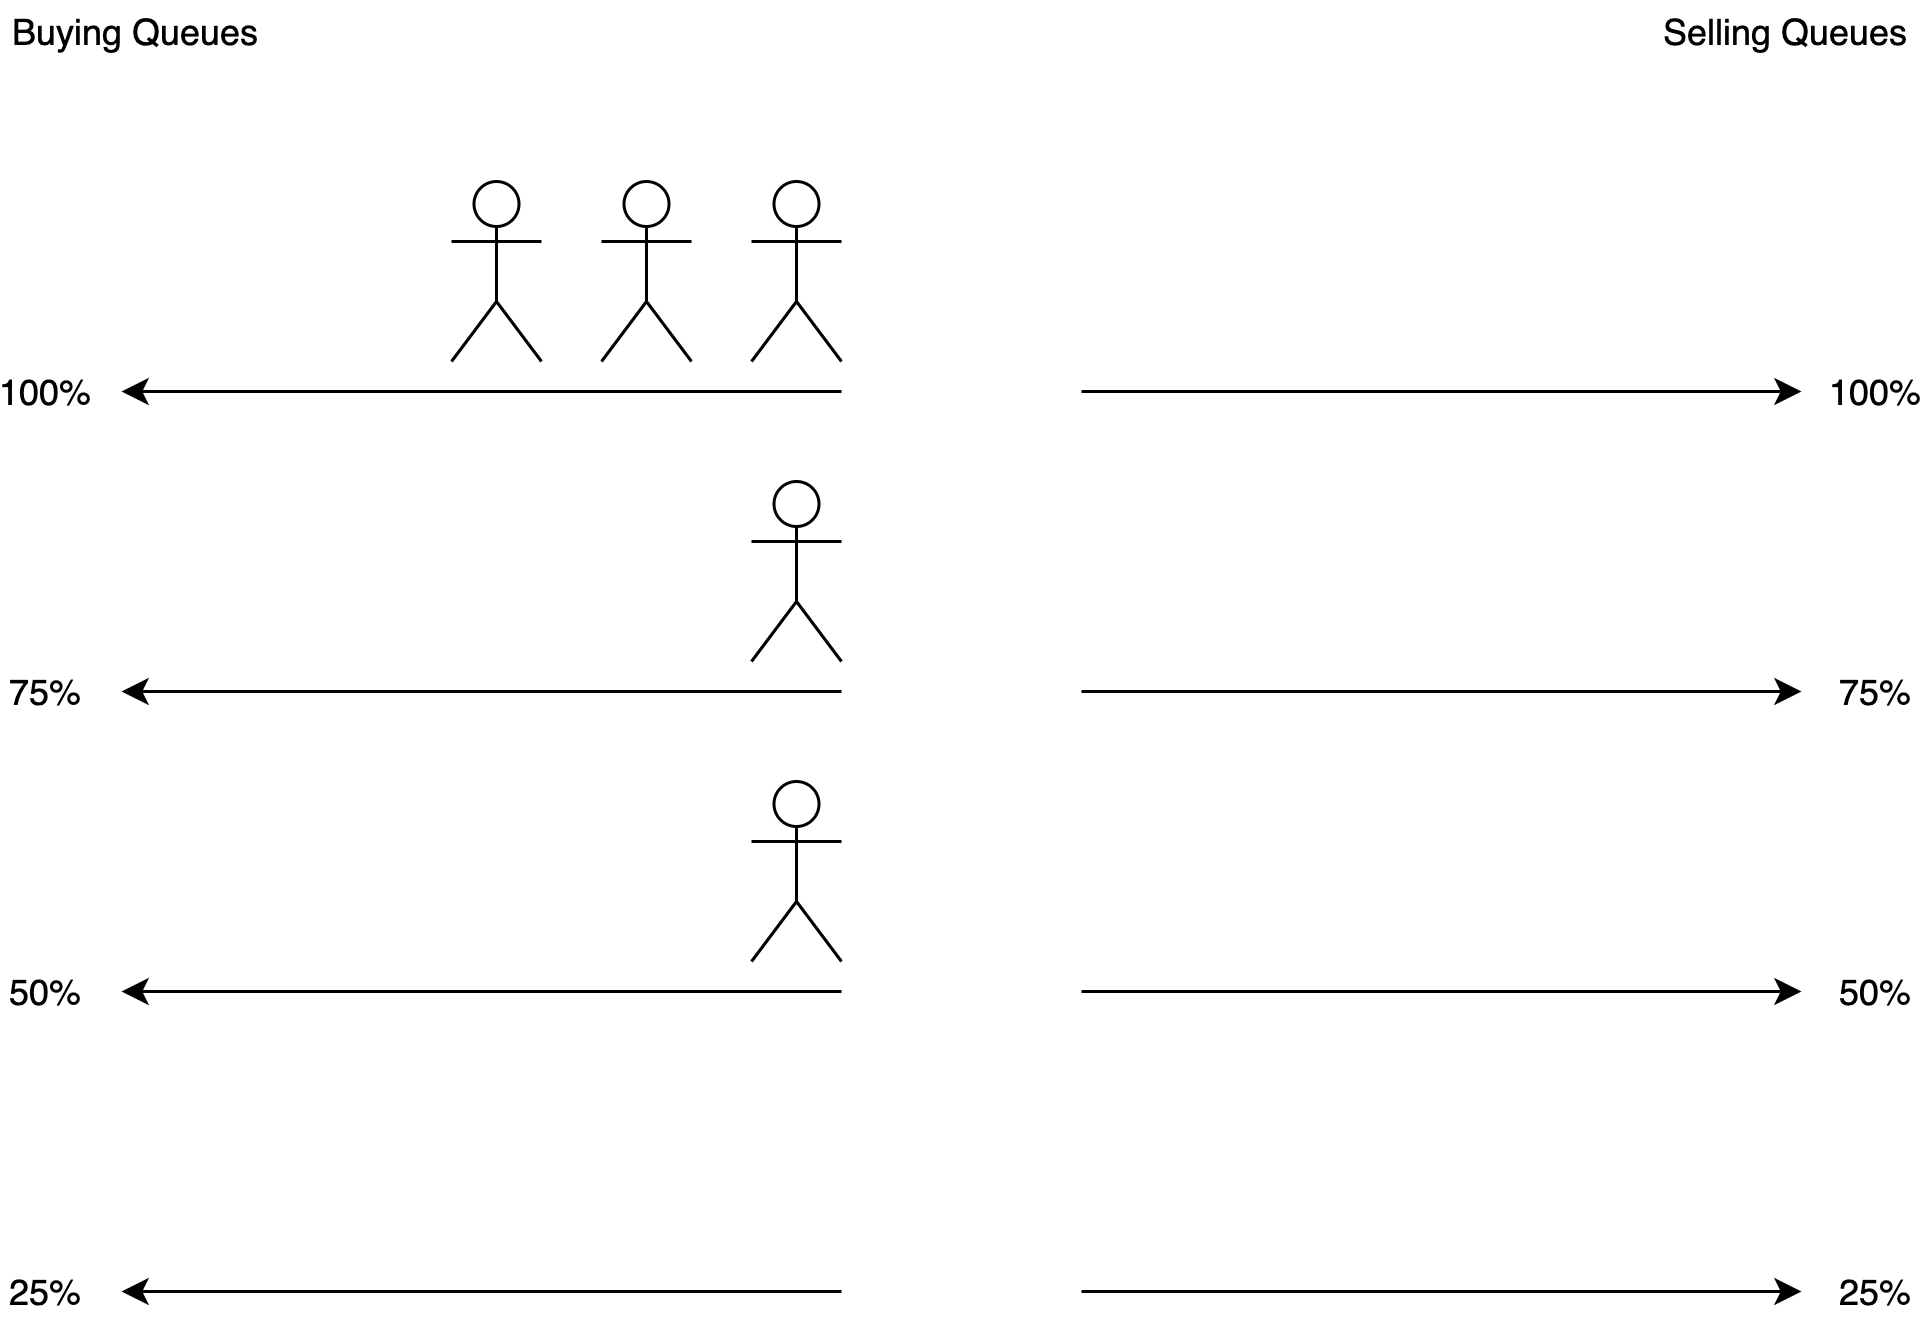
\includegraphics[width=16cm]{figures/aftermarket-high-demand.png}
    \caption{Aftermarket with high demand}
    \label{fig:aftermarket-high-demand}
\end{figure}

It is also possible that the aftermarket levels at a lower price than the original ticket price. This is shown in Figure \ref{fig:aftermarket-mixed} where multiple people are willing to sell the ticket for 75\% of the original price. On the other side, multiple people are willing to buy a ticket for only 50\% of the original ticket price. In this state, any seller could immediately settle a trade at 50\% of the original price and any buyer could immediately fill an offer at 75\%. 

\begin{figure}[H]
    \centering
    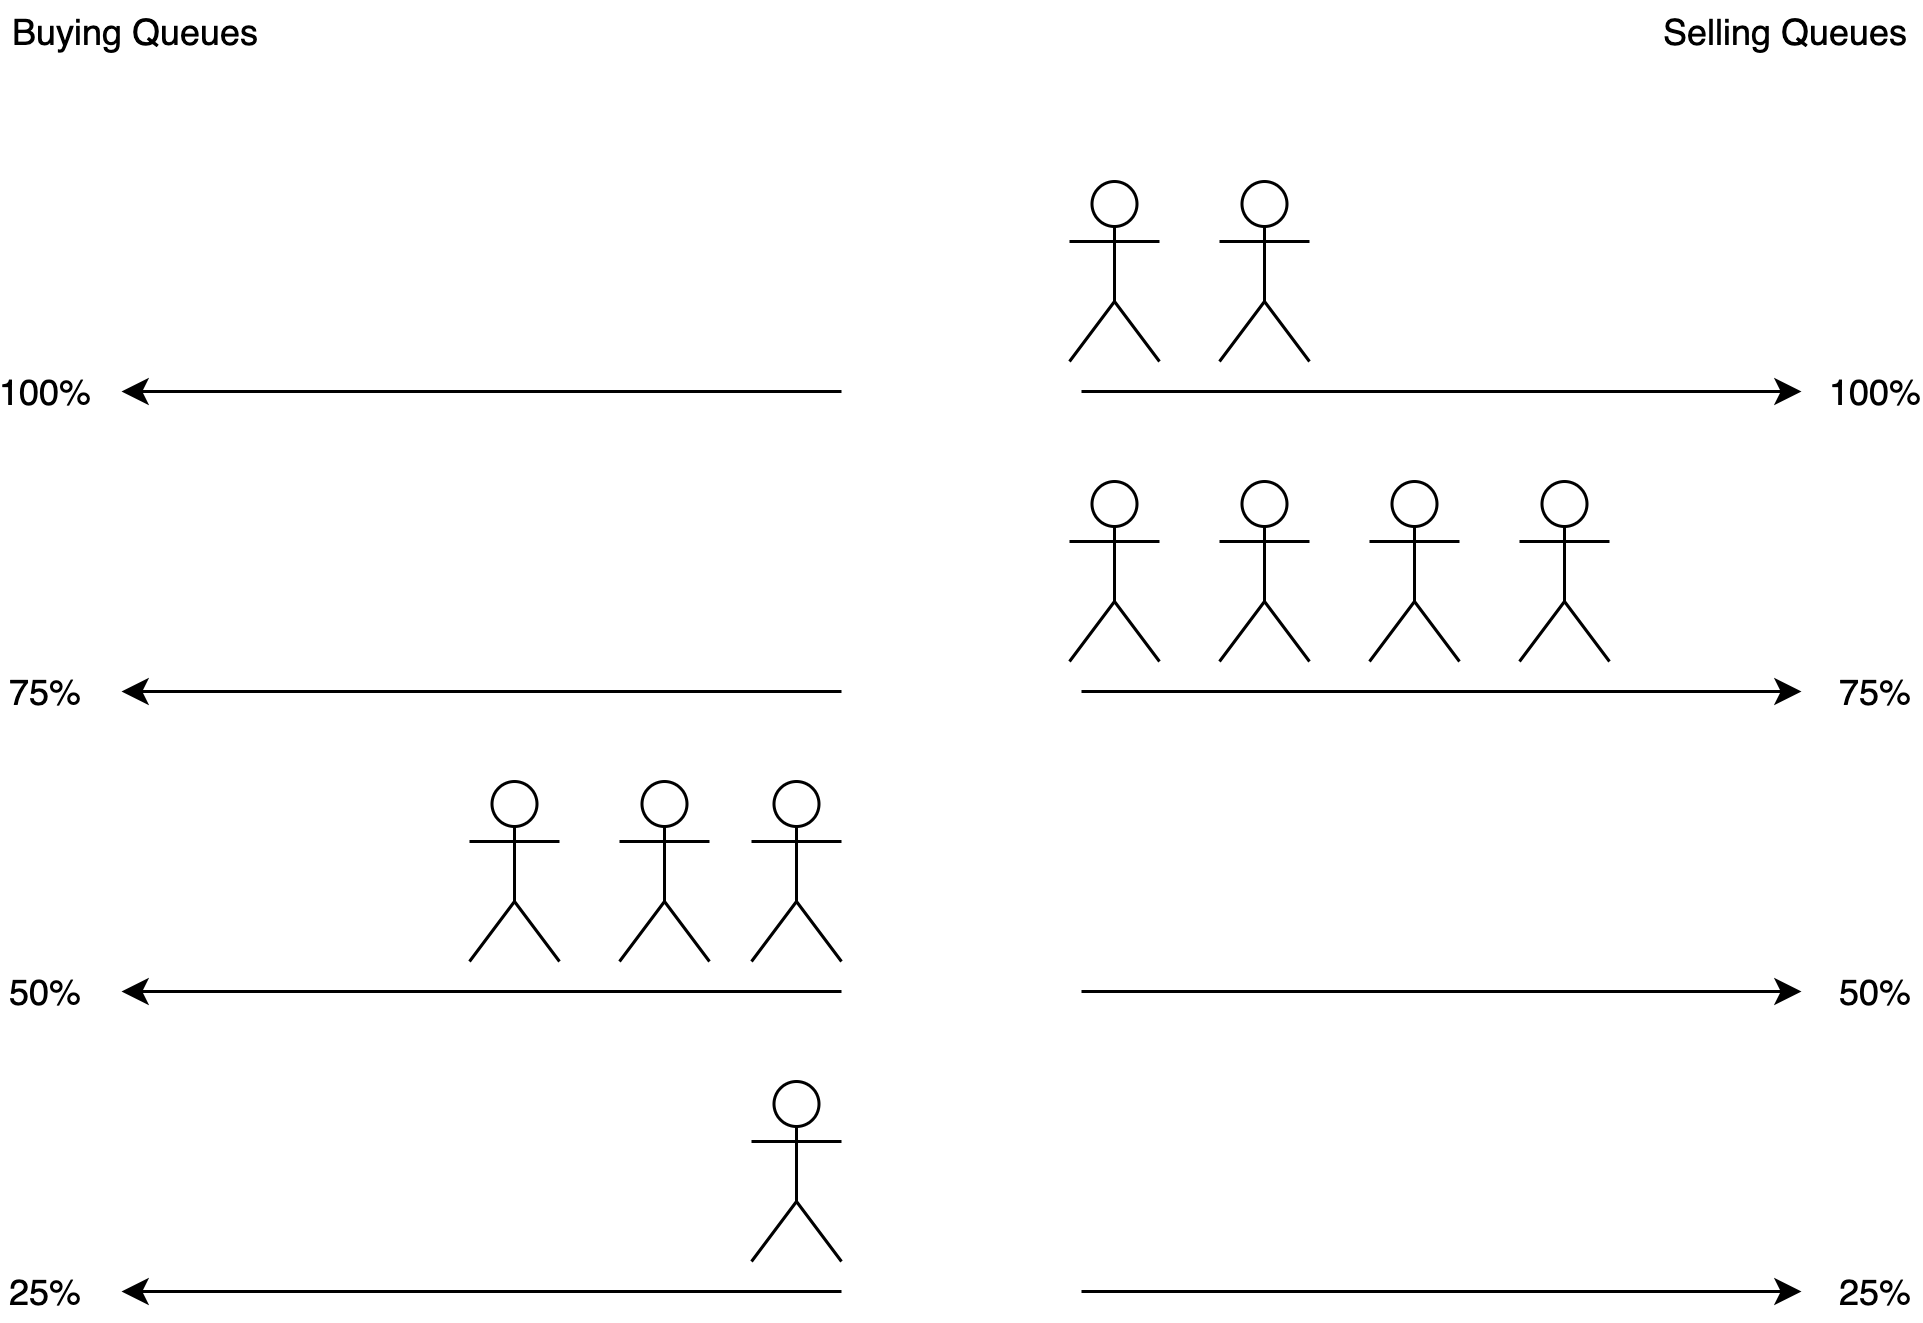
\includegraphics[width=16cm]{figures/aftermarket-mixed.png}
    \caption{Aftermarket with lower prices than original ticket price}
    \label{fig:aftermarket-mixed}
\end{figure}

Another scenario that is possible can occur when people join the wrong queue. This can occur when a sell an buy order is processed in the same block or due to wrong interaction with the smart contract. Such a state of the aftermarket is shown in Figure \ref{fig:aftermarket-arbitrage}. There is a person willing to sell a ticket for less highest offer on the buyer side. This opens the possibility of arbitrage trading. A third person can buy the ticket at 50\% and immediately resell the ticket again for 75\%. 

\begin{figure}[H]
    \centering
    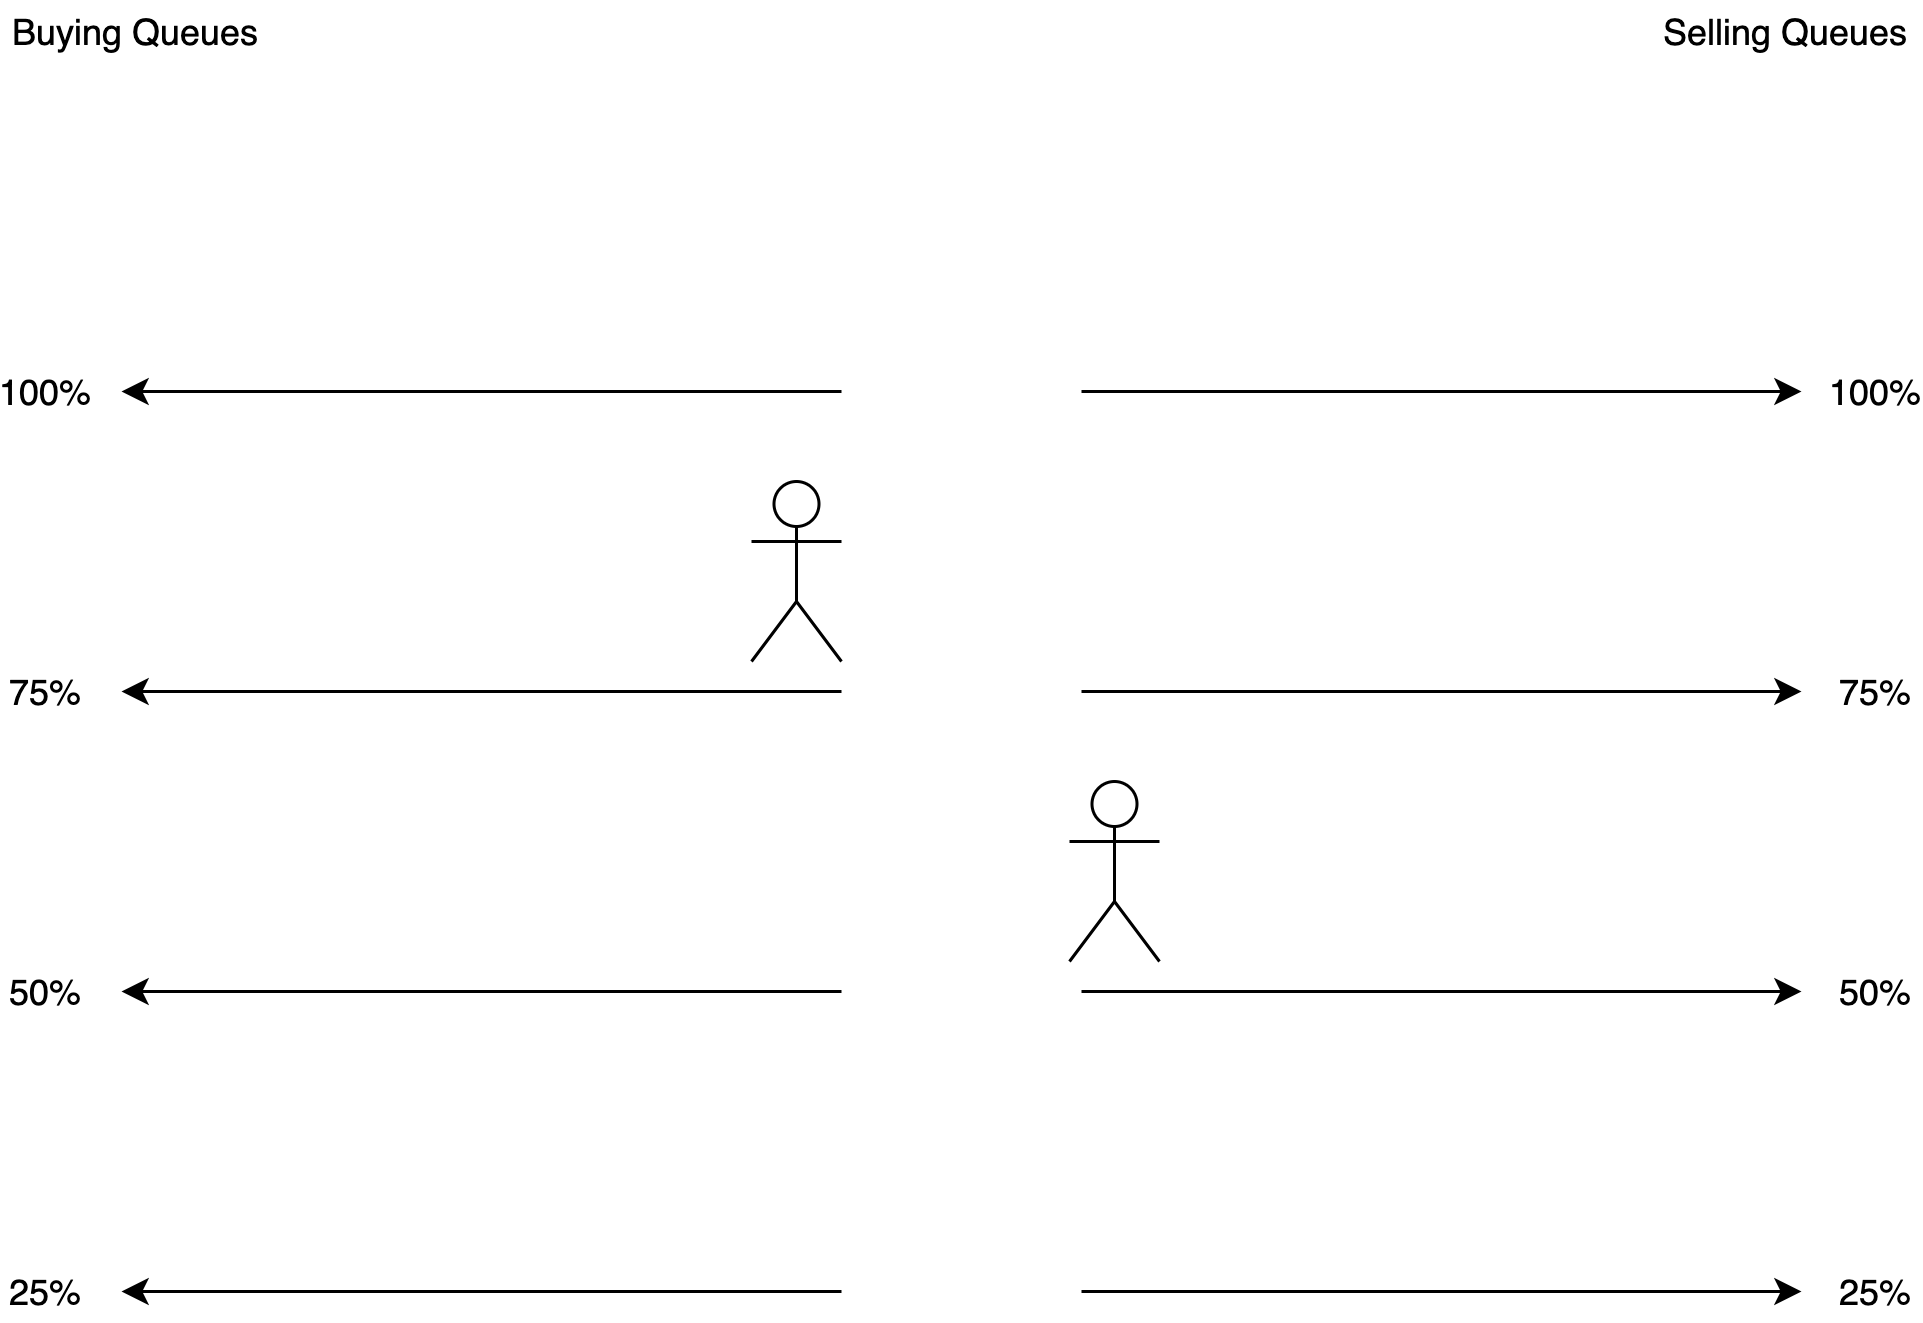
\includegraphics[width=16cm]{figures/aftermarket-arbitrage.png}
    \caption{Aftermarket with arbitrage opportunities}
    \label{fig:aftermarket-arbitrage}
\end{figure}

There are two solutions to solve that problem. Joining the wrong queue due to human error can be eliminated by warning the user in the frontend application that joining the selected queue results in a loss of opportunity cost. 

Solving the issue in the smart contract comes at the price of efficiency. Additional parameter can be introduced to keep track how many people are in each queue. Before each trade, the smart contract evaluates if the described state occurs. However, depending on the granularity of the queues, it might not be feasible to loop over each queue as this results in higher network fees and might lead to an 
\textit{out-of-gas exception}.

In this project, the ... solution was chosen.

\section{ERC standard}
All three ERC standard explained in Section \ref{subsubsection:token-interfaces} require a function which allows the owner to transfer the token/ticket to another address of his choice. Without explicitly deactivating this function, people are to sell the ticket on a different platform for higher prices and consequently, allowing a secondary market to emerge. The goal of this project is that there exists only one marketplace/exchange for each event operating transparently on the blockchain. Also, tickets must not transferred in the same way as these ERC standards do.

It is be possible to deactivate the transfer function or whitelist a specific exchange address such that tickets could only be sold through this exchange. However, this breaks the design principle of these standards. These standards were developed to create a common interface such that a token can be used across multiple exchanges and the usability is the same among different tokens. Also, tickets must only be resold in one contract to minimize the risk of emerging a black market (as described in Section \ref{section:aftermarket}). Merging the event logic with the aftermarket logic in one contract has a positive side-effect that no extra transaction is needed to approve the DEX (aftermarket). 

Furthermore, The logic for approving and storing other exchanges increases the complexity of the event smart contract and becomes more expensive to create deploy a new event.

These are the reason why an event contract does not implement and of the ERC standard interfaces and is bundled as one contract. 